
No agente utilizando MCTS foi aplicado nas escolhas dos jogadores. Uma vez que não é conhecido quais movimentos o Pokémon adversário tem (cada Pokémon pode ter apenas 4 golpes dentre dezenas de golpes que cada diferente Pokémon pode aprender), ficaria muito custoso criar um ramo para cada possível golpe de cada Pokémon (o Pokémon da Espécie Mew por exemplo, tem disponível mais 120 diferentes movimentos).

Os grupos de movimentos implementados foram os seguintes:

\begin{itemize}
	
	\item \textbf{Grupo A}: Utilizar golpe de dano super efetivo. Um golpe super efetivo é um golpe que recebe um acréscimo de $ 2 \times$ ou $ 4 \times$ de sua base de ataque de acordo com o tipo do golpe e do tipo do Pokémon atingido (definido por um sistema de vantagens e desvantagens explicadas no capítulo ???).
	
	\item \textbf{Grupo B}: Utilizar outro golpe de dano qualquer.
	
	\item \textbf{Grupo C}: Utilizar golpe de alteração de estado. Golpe de alteração de estado podem ser golpes que enfraqueçam o inimigo, fortaleça um aliado ou aplique um estado negativo (paralisar, envenenar e etc).
	
	\item \textbf{Grupo D}: Trocar para algum Pokémon que tenha algum golpe super efetivo (Grupo A) contra o atual inimigo.
	
	\item \textbf{Grupo E}: Trocar para outro Pokémon qualquer.
	
\end{itemize}

Antes de cada possível golpe ser encaixado em cada grupo é verificado a imunidade do Pokémon adversário a esse golpe. Caso o Pokémon adversário seja imune ou o golpe não tenha efeito (como por exemplo, curar quando os pontos de vidas já estão 100\%, tentar aplicar o estado de paralização em um Pokémon já paralisado, entre outros) o movimento é descartado não entrando para nenhum grupo.

Caso um grupo não contenha nenhuma ação o grupo é descartado da fase de seleção e expansão do MCTS. No caso de existir mais de uma ação, a escolha é feita diferente para cada grupo, conforme as seguintes regras:

\begin{itemize}
	
	\item \textbf{Grupo A e B}: é definido por qual golpe tem maior dano bruto (dano antes das reduções). Definido pela equação:
	
	\begin{equation}
		danobruto = efetividade \times stab \times baseforca
	\end{equation}
	
	Onde:
	
		\subitem \textbf{efetividade}: $\frac{1}{4}$ (super não efetivo), $\frac{1}{2}$ (não efetivo), $1$, $2$ (efetivo) e $4$ (super efetivo).
		
		\subitem \textbf{stab}: $1$ caso o tipo do Pokémon seja diferente do tipo do golpe e $2$ caso sejam do mesmo tipo.
		
		\subitem \textbf{baseforca}: Força base do golpe.
	
	\item \textbf{Grupo C}: Escolhido aleatoriamente.
	
	\item \textbf{Grupo D e E}: Maior quantidade de HP e depois a maior quantidade do atributo velocidade.
	
\end{itemize}

\subsection{Trabalhos relacionados em MCTS}

Outras implementações podem citadas como o Online Outcome Sampling (OOS) (\cite{Lanctot2014}) ou utilizando Regret Matching junto com MCTS (\cite{tak2014monte}



%Diferente dos jogos de turnos tradicionais onde temos turnos sequenciais uniformes, ou seja, primeiro o jogador A depois o B até que o jogo termine, em batalhas Pokémon as escolhas são feitas simultaneamente e a ordem de execução das ações escolhidas depende de atributos do Pokémon, da ação escolhida e outros efeitos especiais. Segundo \cite{tak2014monte} o algoritmo de MCTS que obteve maior sucesso em jogos com turnos simultâneos é o UCT dissociado.%

Na figura \ref{fig:treePolicy} (\cite{gelly2011monte}) é mostrado cinco simulações do algoritmo MCTS e a relação entre a política de árvore e política padrão. O resultado é igual a 1 se o jogador de cor preta vencer e 0 caso branco vencer. Dentro do nó contém pontuação no formato vitória/visitas.

\begin{figure}[p]
\centering
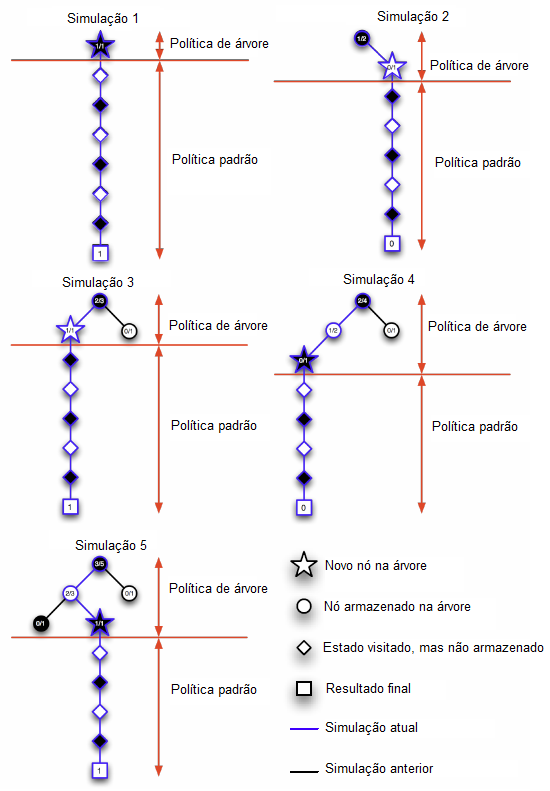
\includegraphics[width=16cm]{figures/politicasMCTS.png}
\caption[Políticas MCTS]{Política de árvore e política padrão.}
\label{fig:treePolicy}
\end{figure}